\documentclass[11pt,letterpaper]{article}

% Load some basic packages that are useful to have
% and that should be part of any LaTeX installation.
%
% be able to include figures
\usepackage{graphicx}
% get nice colors
\usepackage{xcolor}

% change default font to Palatino (looks nicer!)
\usepackage[latin1]{inputenc}
\usepackage{mathpazo}
\usepackage[T1]{fontenc}
% load some useful math symbols/fonts
\usepackage{latexsym,amsfonts,amsmath,amssymb}

% comfort package to easily set margins
\usepackage[top=1in, bottom=1in, left=1in, right=1in]{geometry}

% control some spacings
%
% spacing after a paragraph
\setlength{\parskip}{.15cm}
% indentation at the top of a new paragraph
\setlength{\parindent}{0.0cm}

\begin{document}

\begin{center}
\Large
Ay190 -- Worksheet 2\\
John Pharo\\
Date: \today
\end{center}

\section*{Problem 1}

The following is the copied output of the Python file problem1.py.

\[
\begin{array}{lllllllllllllllll}
n & x_n & \text{Absolute Error} & \text{Relative Error} \\
0 & 1.0 & 0.0 & 0.0 \\ 
1 & 0.333333 & 9.93410748107e-09 & 2.98023224432e-08 \\ 
2 & 0.111111 & 5.29819064732e-08 & 4.76837158259e-07 \\ 
3 & 0.0370373 & 2.16342784749e-07 & 5.84125518823e-06 \\ 
4 & 0.0123466 & 8.71809912319e-07 & 7.06166028978e-05 \\ 
5 & 0.00411871 & 3.48814414362e-06 & 0.0008476190269 \\ 
6 & 0.00138569 & 1.39522571909e-05 & 0.0101711954921 \\ 
7 & 0.000513056 & 5.58089223023e-05 & 0.122054113075 \\ 
8 & 0.000375651 & 0.000223235614917 & 1.46464886947 \\ 
9 & 0.000943748 & 0.000892942551319 & 17.5757882376 \\ 
10 & 0.00358871 & 0.00357177023583 & 210.909460655 \\ 
11 & 0.0142927 & 0.0142870812639 & 2530.91358466 \\ 
12 & 0.0571502 & 0.0571483257835 & 30370.9634027 \\ 
13 & 0.228594 & 0.228593318278 & 364451.584977 \\ 
14 & 0.914374 & 0.914373307961 & 4373419.18641 \\ 
15 & 3.65749 & 3.6574932832 & 52481030.9737 \\ 
\end{array}
\]

Notice that, for n=15, the absolute error is almost the size of $x_{15}$, and consequently, the relative error is huge.

\section*{Problem 2}

See Figure 1 for the plot of the absolute errors $f'(x;h_i) - f'(x)$ for the forward and central difference approximations. Note that, when changing from $h_1$ to $h_2$, the forward difference changes by one factor of the ratio of the step sizes (so $n=1$), but the central difference changes by the ratio squared (so $n=2$). Thus, the forward difference is first-order convergent and the central difference is second-order convergent.

\section*{Problem 3}

The notes calculate the central finite difference approximation by subtracting the forward and backward Taylor expansions and solving for the first derivative. We want a second-order central approximation for the second derivative, which means the final error term must be divided by the coefficient of the second derivative and still end up $O(h^2)$. Thus we make our Taylor expansions

$$ f(x+h) = f(x) + h f'(x) + \frac{h^2}{2}f''(x) + \frac{h^3}{6}f'''(x) + O(h^4) $$

$$ f(x-h) = f(x) - h f'(x) + \frac{h^2}{2}f''(x) - \frac{h^3}{6}f'''(x) + O(h^4) $$

Adding the two together, the first and third derivatives of $f$ will cancel, allowing us to easily solve for the second derivative.

$$ f''(x) = \frac{f(x+h) + f(x-h) - 2f(x)}{h^2} + O(h^2) $$

So we have a second-order central finite difference approximation of the second derivative.

\begin{figure}[!htb]\centering
  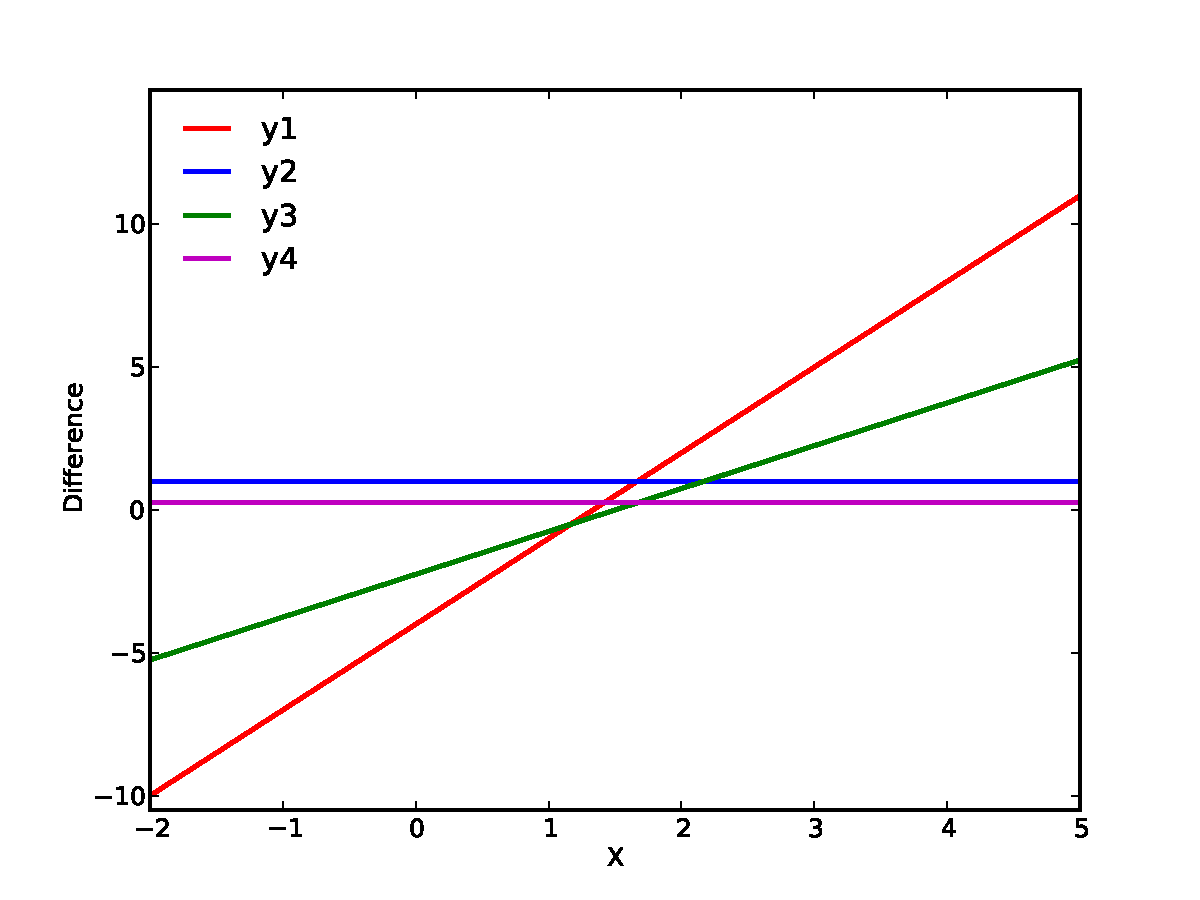
\includegraphics[width=1\textwidth]{FinDifApprox}
  \caption{Plot of the absolute error of the forward and central difference approximations at $h_1$ and $h_2$. $y_1$ and $y_3$ ar ethe forward difference at $h_1$ and $h_2$, and $y_2$ and $y_4$ are the central difference approximations.}
  \end{figure}

\begin{figure}[!htb]\centering
  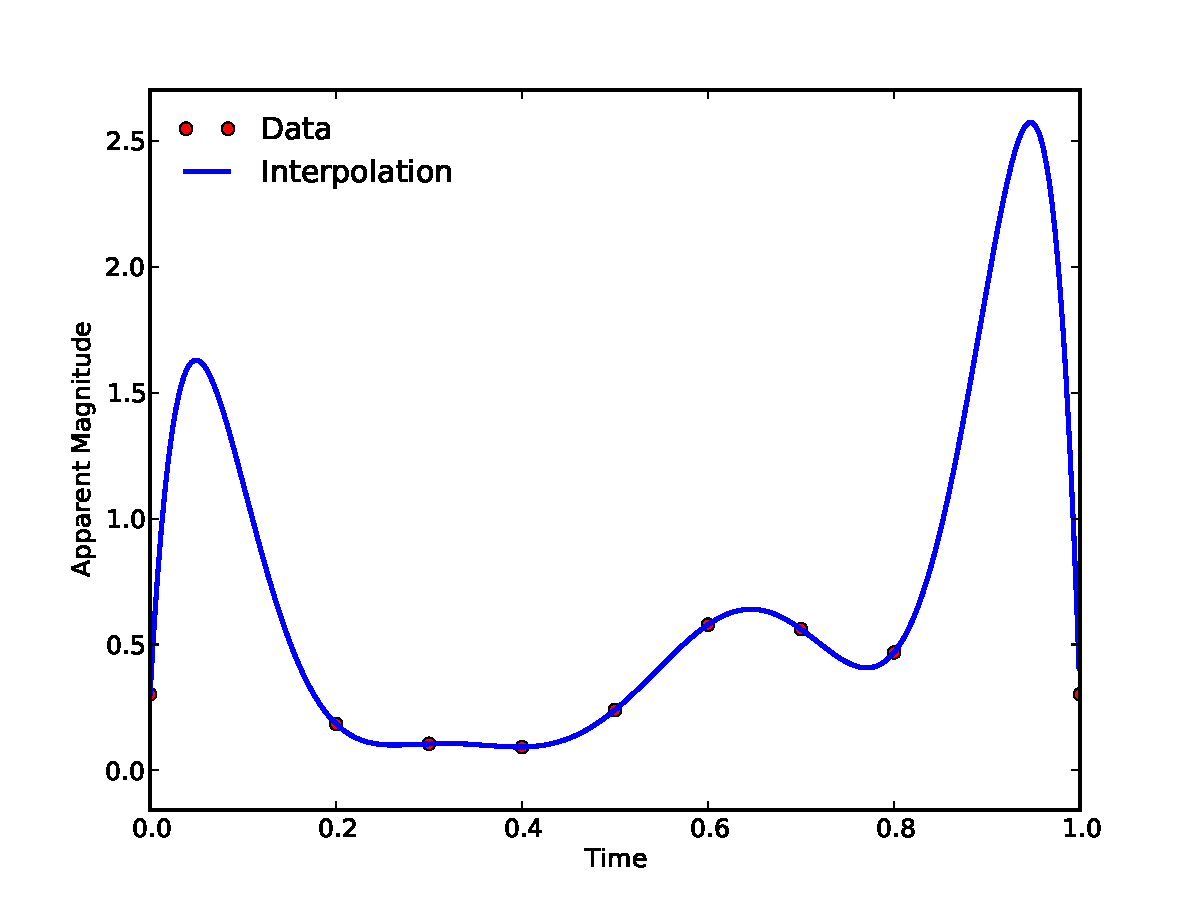
\includegraphics[width=1\textwidth]{Lagrange}
  \caption{A Plot of the 8th-degree global Lagrange interpolation polynomial against the data points provided. Note that the interpolation matches well near the center of the interval, but it gets a bit wild near the edges.}
  \end{figure}

\begin{figure}[!htb]\centering
  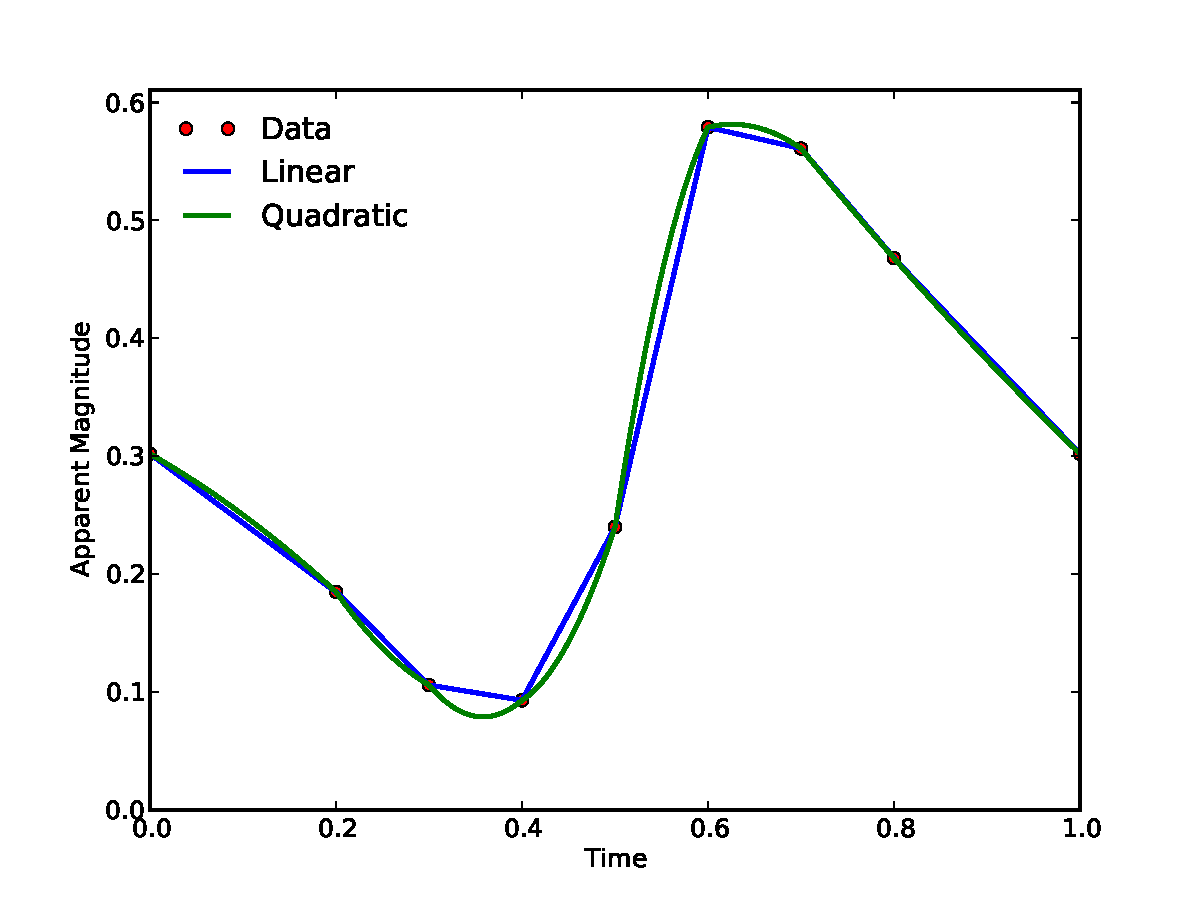
\includegraphics[width=1\textwidth]{Piecewise}
  \caption{A plot of piecewise linear and piecewise quadratic interpolations against the data.}
  \end{figure}

\begin{figure}[!htb]\centering
  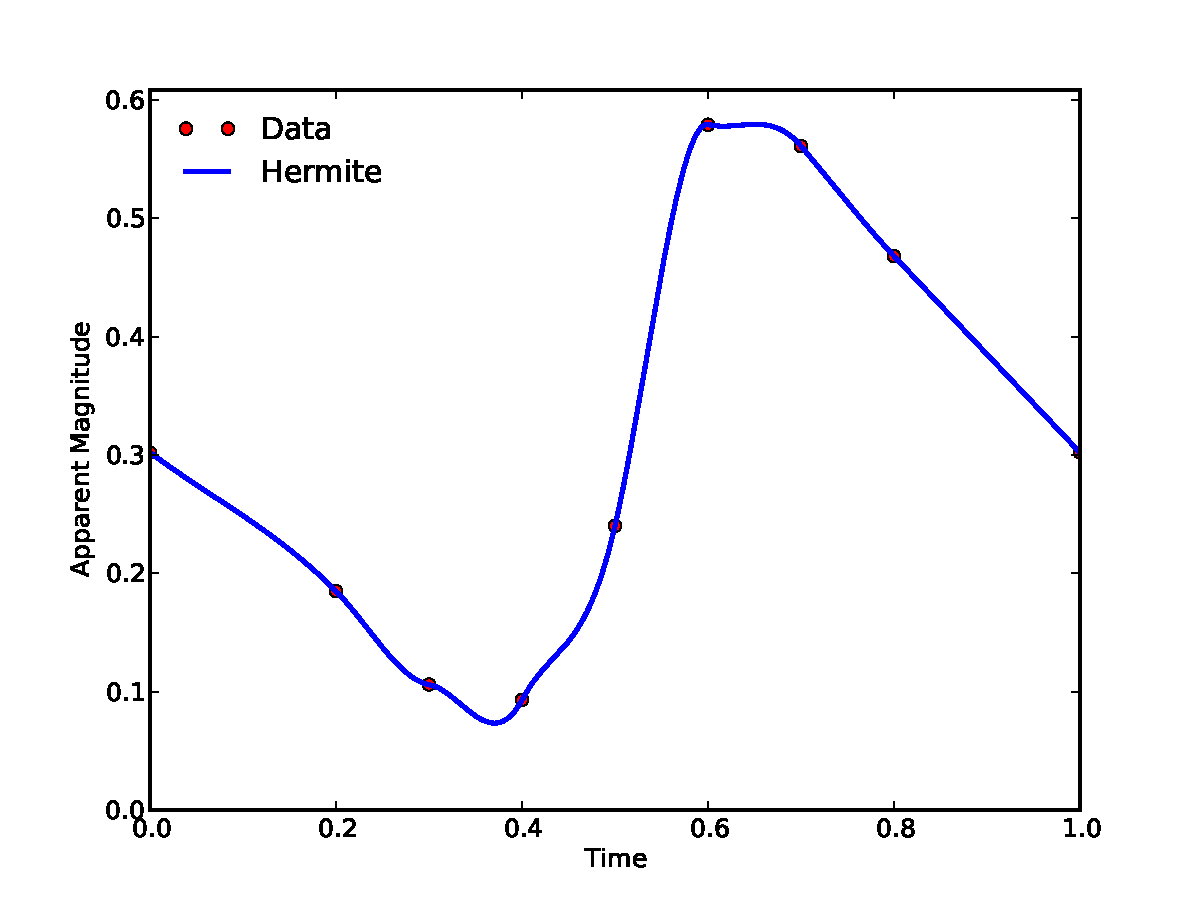
\includegraphics[width=1\textwidth]{Hermite}
  \caption{A plot of a piecewise cubic Hermite interpolation against the data.}
  \end{figure}

\begin{figure}[!htb]\centering
  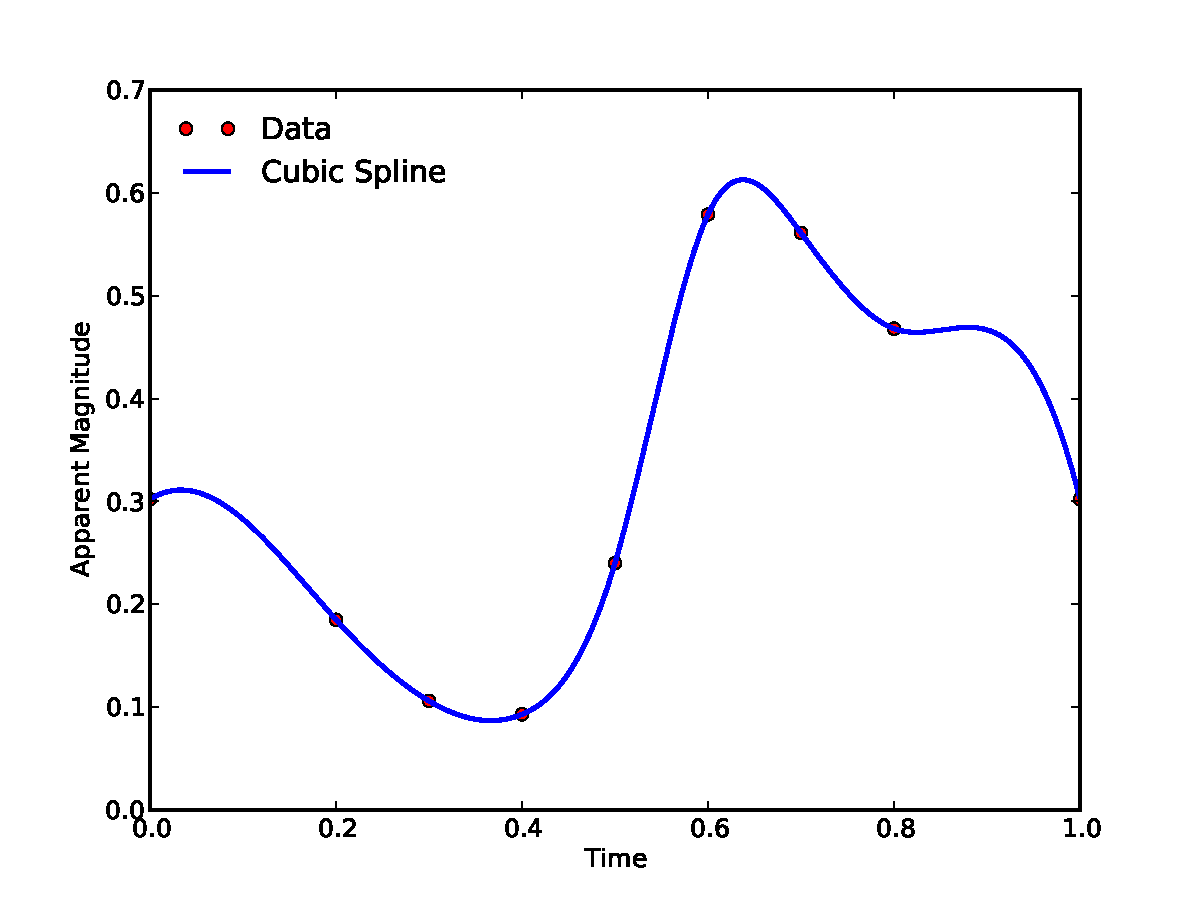
\includegraphics[width=1\textwidth]{Spline}
  \caption{A plot of a natural cubic spline interpolation against the data, using scipy's interp1d function.}
  \end{figure}

\end{document}
